
\documentclass[10pt, twocolumn]{article}
\usepackage{amsmath}
\usepackage{siunitx}
\usepackage{graphicx, float}
\usepackage[plain]{algorithm}
\usepackage[strings]{underscore}
\usepackage{url}
\usepackage{hyperref}

\topmargin=-0.45in
\evensidemargin=0in
\oddsidemargin=0in
\textwidth=6.5in
\textheight=9.0in
\headsep=0.25in


\title{Group Design Project: Formal Report}
\author{Alex Booth}



\begin{document}
    \maketitle

    \section{Introduction}
        
    \section{Background and Theory Basis}
        \subsection{Introduction}
            For a building to function as both a music studio and as an educational facility, special considerations must be taken.
        \subsection{Educational facilities}
            Any building that facilitates or is used for educational purposes must comply to the education building regulations specified by the government.
            These specifications are laid out in Building Bulletin 93 (BB93): Acoustic design of schools - performance standards.
            The importance of acoustic considerations is given by the National Education Union: "Noise from adjacent rooms disrupts the learning process, especially during quiet reading times or test-taking"\cite{NEU}
            The NEU further states the importance of tuning the reverb time of a classroom environment such that the teacher can be heard clearly at any point the classroom, but also so that the conversation of students does not descend into cacophony.
            In BB93, a table of appropriate $L_{AEQ}$ values are given for various classrooms.
            In this context, only the music rooms and common rooms entries are relevant.
            \begin{figure*}
                \centerline{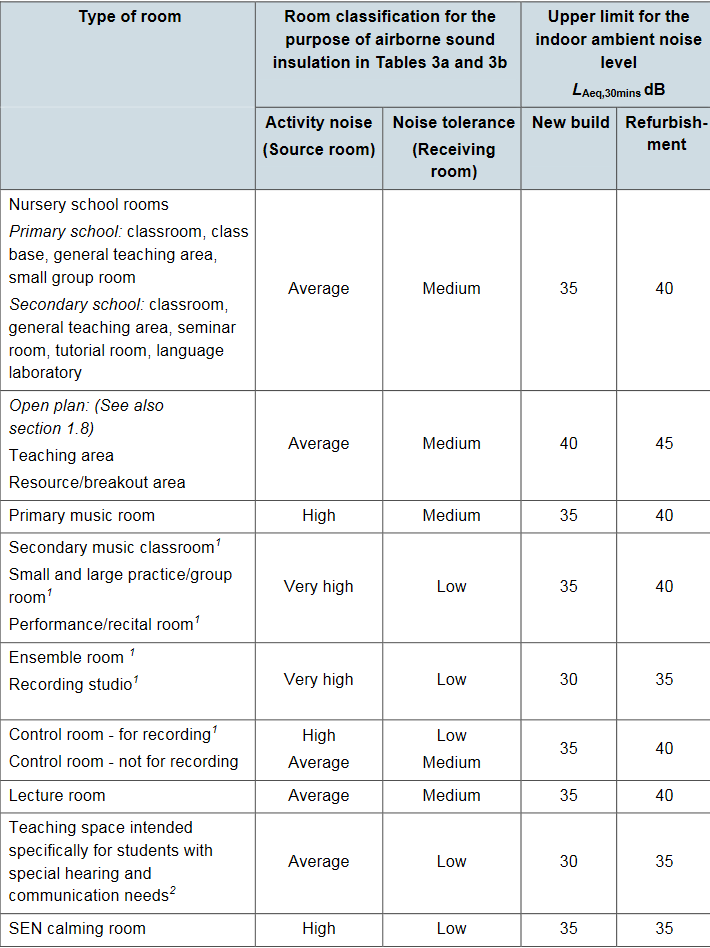
\includegraphics[scale = 1]{resources/BB93.png}}
                \caption{The tabulated $L_{AEQ}$ requirements of an educational environment}
                \label{BB93}
                \centering
            \end{figure*}
            In Fig.\ref{BB93} it can be seen that classrooms and general teaching rooms have a matching ambient noise requirement to lecture rooms.
            The live room in the studio complex can function not only as a live room for large ensemble recordings but also as a class / lecture room.
            Furthermore, the control rooms, isolation rooms and foley rooms will be able to function as SEN calming rooms and teaching space for those with special hearing a communication needs, as they provide the acoustically 'dead' environment specified in the table, with a low ambient noise level.

        \subsection{Music and Recording Facilities}
            Mainstream music education at a secondary level primarily focuses on basic music theory of rhythm, timbre and tone, along with basic music technology requirements.
            In the live room, large ensemble performances and lecture-style teaching can take place, whilst students wishing to practice any instruments can use the iso and control rooms to be isolated from the noise of the live room, and vice versa for the students in the live room.
            For later years of education, the studio will be able to function as an excellent teaching environment for students of sound recording techniques and studio production, with three separate control rooms and one mastering room all equipped such that they can all be used for mixing and mastering.

    \section{Building Layout}

        The floor plan of the envisioned building is illustrated in Fig.\ref{floorplan}:
        \begin{figure*}
            \centerline{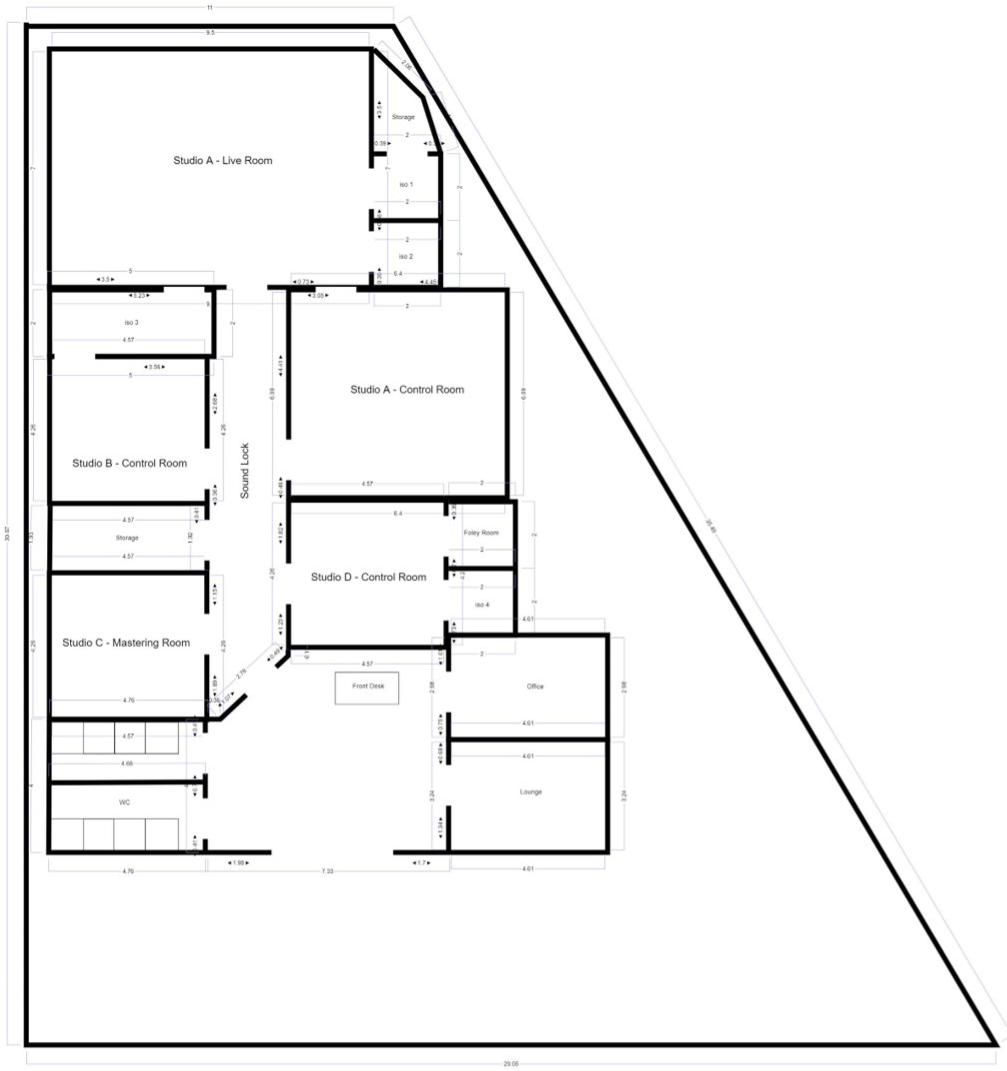
\includegraphics[scale = 0.8]{resources/floorplan.png}}
            \caption{The floor plan of the music educational facility}
            \label{floorplan}
            \centering
        \end{figure*}
        With only one regular point of entry and exit, any entrances or exits made by students or staff can be monitored, such that issues with missing equipment or safeguarding concerns can be easily managed.
        Studio A has a transparent viewport into the live room.
        Thus, it can be used as a control room for any large ensemble recording, such as an orchestra.
        The same applies for the viewport between iso room 3 and the live room.
        It is important to consider the AV-over-IP networking technology used by the studio; it allows for fluid redirecting of the signal chain in a recording environment.
        For example, the live room can be also be used as a control room for a recording in iso room 3, with minimal adjustment to the hardware present in either room.
        All that may need to be changed is the software patching of the AV-over-IP.
        This further allows any student to become proficient in using AV-over-IP technology, a fast advancing technology in the modern studio environment.
        
    \section{Noise Criteria}
        Unwanted noise both from within the studio and from without is an issue of great consideration for recording studios.
        A potentially perfect take can be ruined by microphone bleed of a truck passing by or an underground train shaking the floor.
        The most effective method for preventing noise from entering a room is designing the structure of the room such that the vibrations travelling through solids and sound waves causing said unwanted noise are prevented from entering the structure.
        This can prove challenging, as acoustic waves can travel through almost any solid of a reasonable structural thickness, and a solid structure is by far the easiest and most common way to design the built environment.
        In anechoic chambers found in acoustic research institutes, rooms are suspended from large mass dampers within rooms, with the chamber having a completely separate set of foundations from the rest of the building. REF.
        This construction and design, whilst incredibly effective at reducing outside noise from coming into a room, is very costly and restrictive.
        Instead, our studio was acoustically designed with the aim of reducing outside noise, whilst still providing a familiar built environment.
        Elements we considered included: Absorption, damping, decoupling and distance.
        Absorption of unwanted noise can be achieved by placing acoustic insulation between each wall section, as illustrated in Fig.\ref{wallFiller}
        \begin{figure}[H]
            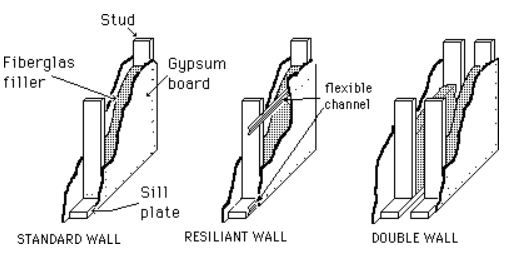
\includegraphics[scale = 0.6]{resources/wallFiller.png}
            \caption{Filling wall partitions with acoustic insulation \cite{UCSC}}
            \label{wallFiller}
            \centering
        \end{figure}

    \section{Acoustic Parameters}

    \section{Noise Insulation}

    \section{Studio Layout}

    \section{Location case study}

    \section{Conclusions}

    \bibliographystyle{plain}
    \bibliography{theBib}

\end{document}